\documentclass{article}

\usepackage{amsmath}
\usepackage{listings}
\usepackage{amsfonts}
\usepackage{amssymb}
\usepackage{xcolor}
\usepackage{graphicx}
\usepackage{titling}
\usepackage[utf8]{inputenc}
\usepackage[english]{babel}
\usepackage{amsmath}
\usepackage{fancyhdr}
\usepackage{lastpage}
\usepackage{textcomp}
\usepackage{graphicx}
\usepackage{hyperref}
\usepackage{float}

\addtolength{\oddsidemargin}{-.875in}
\addtolength{\evensidemargin}{-.875in}
\addtolength{\textwidth}{1.75in}
\addtolength{\topmargin}{-.875in}
\addtolength{\textheight}{1.75in}

\title{\Huge System Management \vspace{1cm}}
\author{Riccardo Biella, Elia Perrone, Nicolas Sala, Kevin Dominguez}
\date{Semestre primaverile 2019}
\setcounter{page}{0}
\pagestyle{fancy}
\fancyhf{}

\fancyfoot[C]{Page \thepage \hspace{1pt} of \pageref{LastPage}}


\begin{document}
\maketitle
\thispagestyle{empty}
\pagebreak

\tableofcontents
\lstset{language=C++}
\pagebreak

\section{Esercitazione 01}

\begin{figure}[H]
    \center
    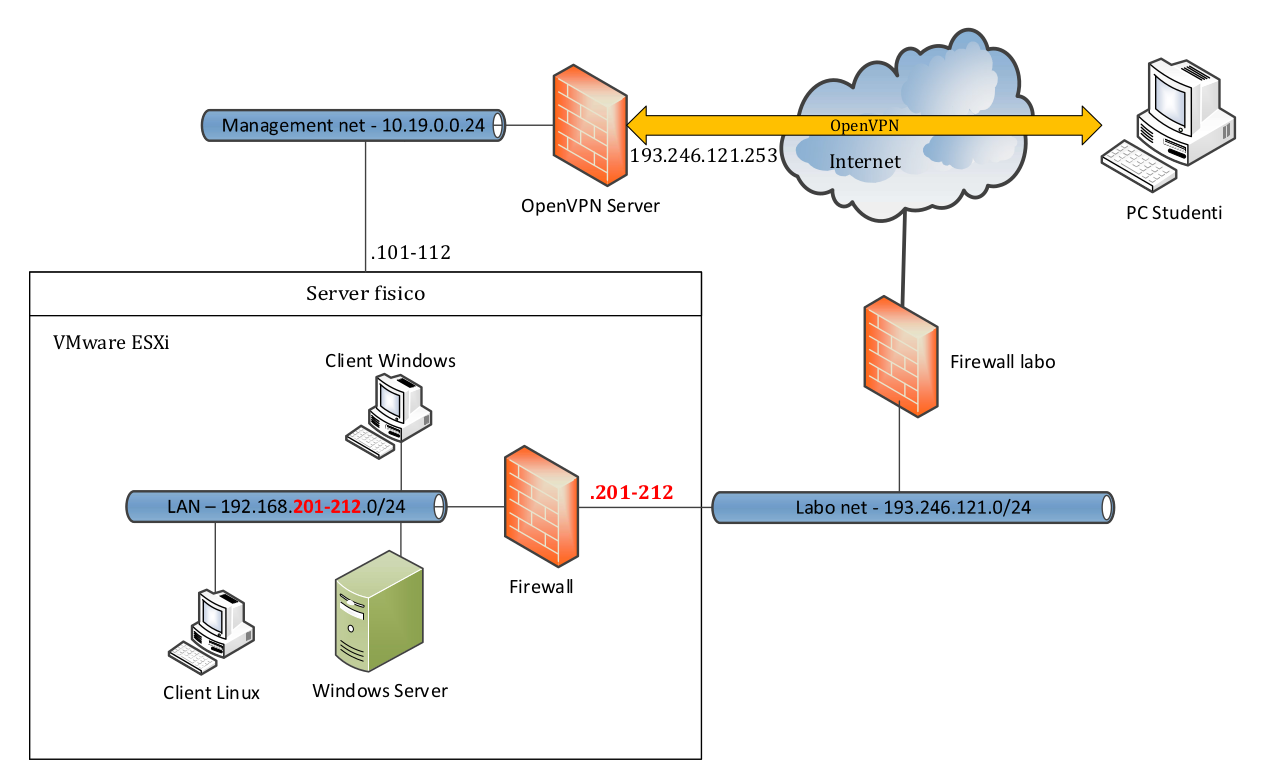
\includegraphics[scale=0.3]{images/schemaRete.png}
    \caption{Schema di rete base}\label{fig:1}
\end{figure}

\subsection{Specifiche del server utilizzato (Gateway GW2000h-GW170hq F1)}
Il server utilizzato per le esercitazioni può contenere fino a quattro nodi, con le seguenti caratteristiche:
\begin{figure}[H]
    \center
    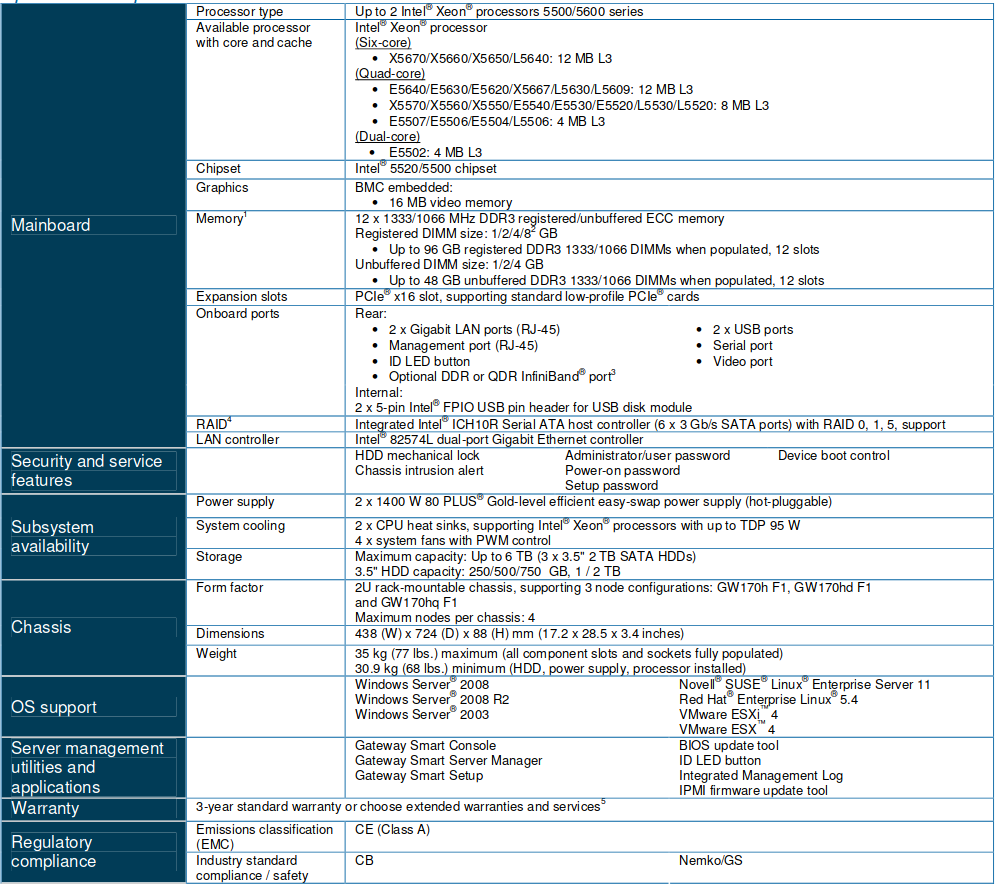
\includegraphics[scale=0.37]{images/specificheServer.png}
\end{figure}

\subsection{Hardware utilizzato}
Ad ogni gruppo è stata assegnata la gestione di un nodo all'interno del rack, esso dispone di un disco rigido, un SSD ed una periferica USB mediante il quale sarà possibile installare un hypervisor sul server.

\subsection{Interfaccia di gestione}
L'interfaccia di management del server, permette la gestione di numerosi aspetti della macchina, tra cui il controllo remoto, che utilizzaremo per lavorare sul server senza essere fisicamente presenti in laboratorio.
L'interfaccia di gestione è raggiungibile all'indirizzo IP: 10.19.0.106, a seguito di una connessione tramite client vpn, con le credenziali seguenti: \\  \textbf{username:} grp6 \\ \textbf{password:} System3m.Man\_grp6
\begin{figure}[H]
    \center
    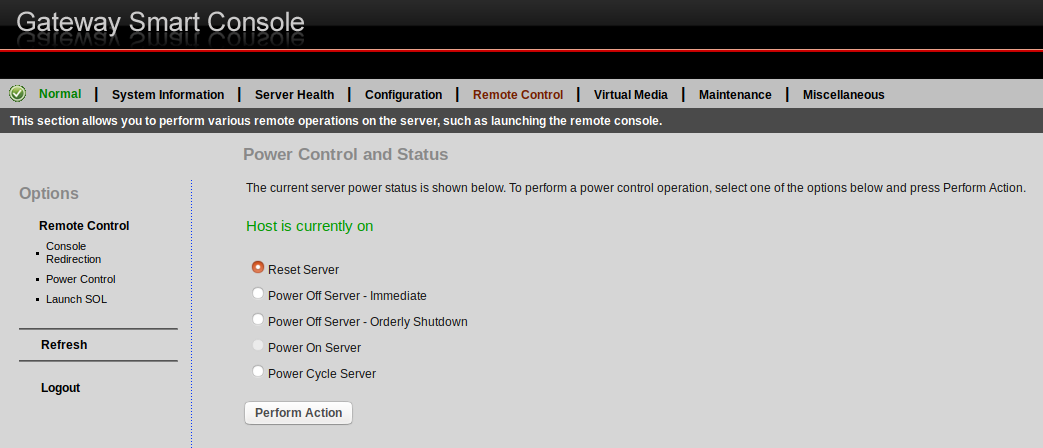
\includegraphics[scale=0.37]{images/GUIManagement.png}
\end{figure}

\subsection{OpenVPN}
\subsubsection{Obiettivo}
Connettersi tramite OpenVPN ed esplorare l’interfaccia di gestione del proprio
server (10.19.0.101-112) (user: root password: superuser) e documentare
azioni e informazioni disponibili.
(Gli account OpenVPN sono gestiti dal docente, che distribuisce ad ogni gruppo
un certificato personalizzato da importare nel proprio OpenVPN client – esempio
di nome di un certificato: SystemManagement-udp-1194-grp5.ovpn e
SystemManagement-udp-1194-grp5.p12).

\subsubsection{Installazione OpenVPN - Ubuntu x64}
\begin{enumerate}
    \item apt-get install openvpn \\ 
    Installiamo openvpn sulla nostra macchina
    \item openvpn --version \\
    Verifichiamo che l'installazione sia andata a buon fine
    \item openvpn --config client.ovpn \\
    Ci posizioniamo nella cartella (unzippata) che abbiamo scaricato da ICorsi,
    avviamo il client con il certificato corretto (.ovpn) che ci è stato fornito.
\end{enumerate}

\subsubsection{Problematiche} 
    Il server mette a disposizione una finestra con la quale è possibile lavorare in modalità
    grafica stile desktop remoto. Tale applicazione fa scaricare un file .JNLP dal server
    (lanciando il controllo remoto dalla console di gestione). Qualora il certificato di
    sicurezza fosse scaduto, si dovrà procedere a creare il trust al server nella macchina
    client (che altrimenti ne blocca l’esecuzione): aggiungere l’IP del server nelle Exception
    Site List di Java. Utilizzando OpenJDK non è possibile sfruttare l'interfaccia grafica di gestione, per questo 
    motivo abbiamo dovuto installare Oracle JRE.

\subsection{VMware ESXi}
\subsubsection{Descrizione}
VMware ESX Server è un prodotto per la virtualizzazione di livello enterprise offerto da VMware Inc., sussidiaria di Dell Technologies e ancor prima una divisione di EMC Corporation. ESX Server è un componente di un'offerta VMware più grande, VMware Infrastructure, che aggiunge servizi di amministrazione e di affidabilità al prodotto base. 
\subsubsection{Architettura}
Il server ESX include un microkernel che si interfaccia direttamente con la macchina. Nelle versioni ESX 3 e precedenti all'avvio viene lanciato un kernel Linux (una versione modificata di Red Hat Enterprise Linux) che analizza l'hardware della macchina e alcuni componenti di gestione, per poi cedere il controllo al componente vmkernel sviluppato di VMware. Questo è un microkernel con tre interfacce verso l'esterno:
\begin{enumerate}
    \item hardware
    \item sistema guest
    \item servizio console (servizio di gestione delle macchine virtuale che gira sul kernel che ha fatto partire vmkernel)
\end{enumerate}

\subsubsection{Installazione di VMWare} 
    Dopo esserci collegati all'interfaccia di gestione della macchina, sulla scheda Remot Control abbiamo scaricato il file .JNLP ed attraverso la sua esecuzione
    abbiamo installato l'hypervisor: abbiamo settato un IP statico pubblico in modo da non dover
    accedere ogni volta tramite VPN. Abbiamo utilizzato per installare VMWare una periferica USB collegata direttamente al server.
    
\subsubsection{Altre opzioni di virtualizzazione}
\begin{enumerate}
    \item VirtualBox (Linux/Mac/Windows)
    \item Parallels (Linux/Mac/Windows)
    \item QEMU (Linux)
    \item Windows Virtual PC (Windows)
\end{enumerate}

\section{Esercitazione 02}

\begin{figure}[H]
    \center
    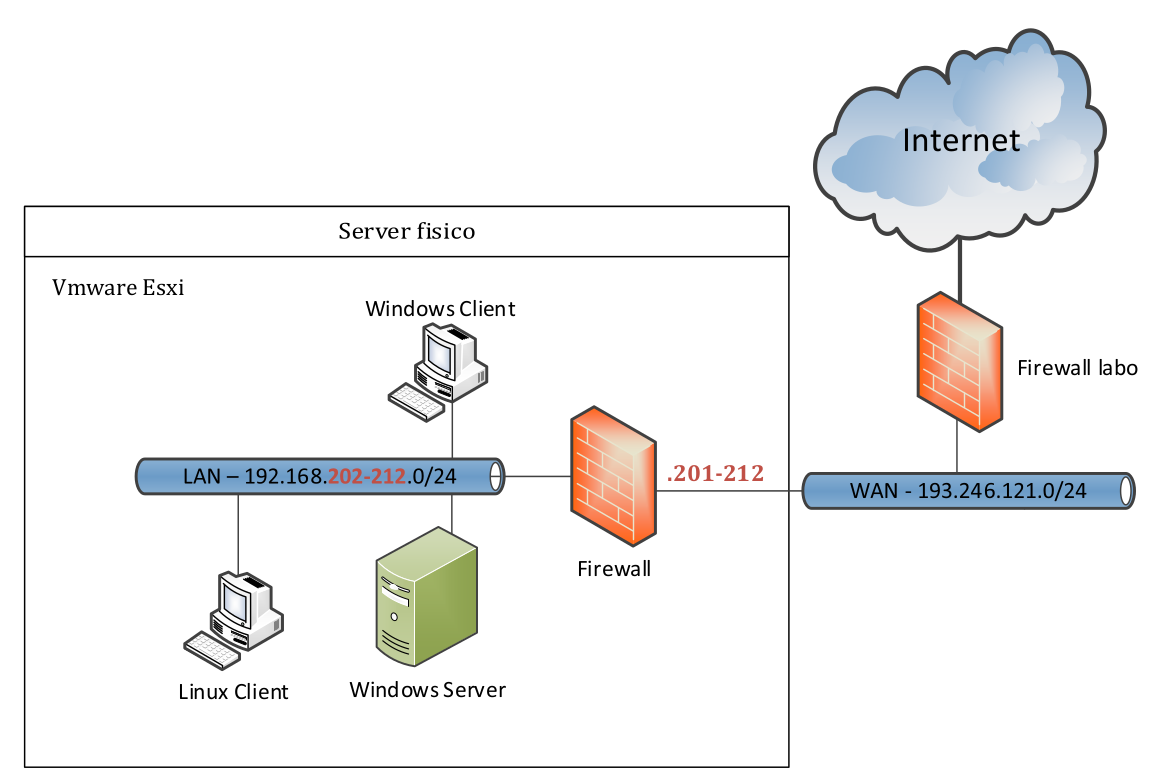
\includegraphics[scale=0.3]{images/s2.png}
    \caption{Schema di rete base}\label{fig:1}
\end{figure}

\subsection{Obiettivo e definizione di una struttura di rete}

\begin{figure}[H]
    \center
    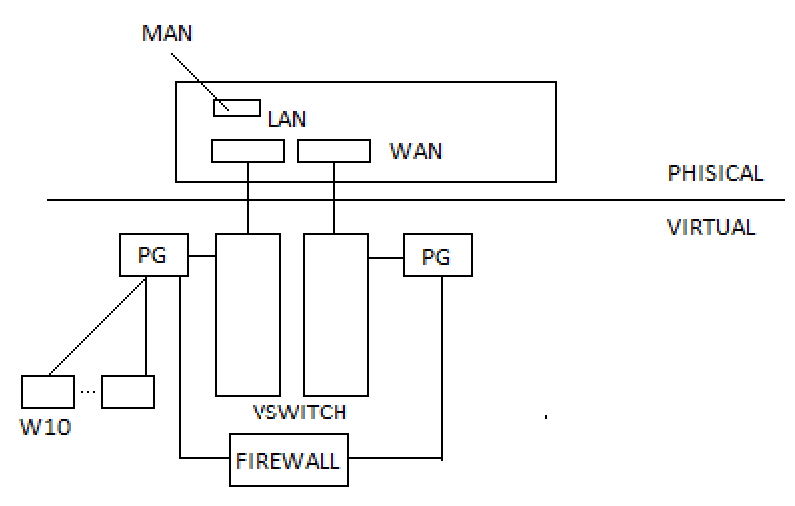
\includegraphics[scale=0.5]{images/lavagna.png}
    \caption{Struttura di rete}\label{fig:1}
\end{figure}

\noindent 
L'obiettivo finale dell'esercitazione è quello di virtualizzare l'intera rete collegata alle interfacce LAN e WAN del server.
Nell' immagine è possibile osservare lo schema di rete che vogliamo realizzare.
Nella parte superiore "Phisical", troviamo il server, con le sue interfacce MAN, LAN e WAN.
Nella parte inferiore "Virtual" definiamo l'infrastruttura di rete che vogliamo virtualizzare. Si osservano due virtual switch, collegati a due
port group, allo stato attuale disponiamo solo di un VS e di un PG, perciò dovremo creare un nuovo VS
collegato all'interfaccia LAN e creare un nuovo port group nuovo collegato al VS creato.
I port group non sono altro che un'astrazione ad un livello più alto degli switch,
su di essi possono risiedere le VLAN.
Nel corso dell'esercitazione procederemo ad installare alcune macchine virtuali client e server e un un firewall che sarà collegato ai port group con due interfacce, una LAN e una WAN (pubblica).
Le macchine virtualizzate saranno poi collegate al nostro nuovo port group. L'indirizzo IP assegnato al nostro firewall
finisce in .236. Sul firewall installeremo poi un client VPN.
Come ultimo passaggio dobbiamo spostare l’interfaccia di gestione di ESXi all’interno della rete (LAN).

% Sulla scheda virtual machine dell'interfaccia pubblica del server abbiamo cliccato su Create / Register VM
% per uplodare un'immagine di una nuova macchina virtuale.

\subsection{Firewall utilizzato}
PFSense è una distribuzione software open source basata su FreeBSD adatta per essere utilizzata come firewall/router. 
Ha lo scopo di fornire un firewall potente, sicuro e completamente configurabile utilizzando l'hardware di un comune PC. Nel cuore del sistema c'è FreeBSD e il firewall PF (Packet Filter) in prestito da OpenBSD da cui deriva appunto il suo nome, che ha il significato di "dare maggior senso per l'utente finale a PF".


\subsubsection{Versione utilizzata e requisiti minimi di sistema}
\textbf{Versione:} PFSense \\
\textbf{Memoria RAM:} 512 MB

\subsubsection{Funzionalità}
Possiede le funzionalità basilari di un firewall di qualità:

\begin{itemize}
    \item Stateful Firewall con controllo granulare e possibilità di funzionare in maniera trasparente al layer 2 (in bridging)
    \item Network address translation
    \item HA (High Availability): grazie a CARP permette di configurare due firewall su due macchine identiche per replicarsi e autosostituirsi nel caso di guasto di una delle due (il software pfsync si occupa di replicare lo stato firewall, la tabella delle connessioni e le regole del firewall, permettendo di passare al secondo firewall senza che le connessioni attive di rete cadano)
    \item Load Balancing: bilanciamento del carico di lavoro tra due o più server che si trovano dietro a pfSense (utilizzato normalmente per web server, mail server, ecc.)
    \item VPN server, su protocolli IPsec, OpenVPN e PPTP.
    \item PPPoE server
    \item Grafici RRD ed informazioni sullo stato in tempo reale.
    \item Captive portal
    \item Gestione uPnP e DNS dinamici
\end{itemize}
Grazie all'aggiunta di ulteriori moduli è possibile estendere le funzionalità di base ed integrarne di evolute come web proxying (con Squid), url filtering (Squidguard, DansGuardian), IDS (Snort) , antivirus (HAVP) ed altre ancora, fino alla gestione di messaggistica VoIP con FreeSWITCH. 

\subsection{Installazione Windows Server 2012}
\subsubsection{Versione utilizzata e requisiti minimi di sistema}
\textbf{Versione:} Windows Server 2012 ???\\
\textbf{Memoria RAM:} 2 GB \\
\textbf{Hard Disk:} 60 GB

\subsubsection{Tabella comparativa delle versioni}
\begin{figure}[H]
    \center
    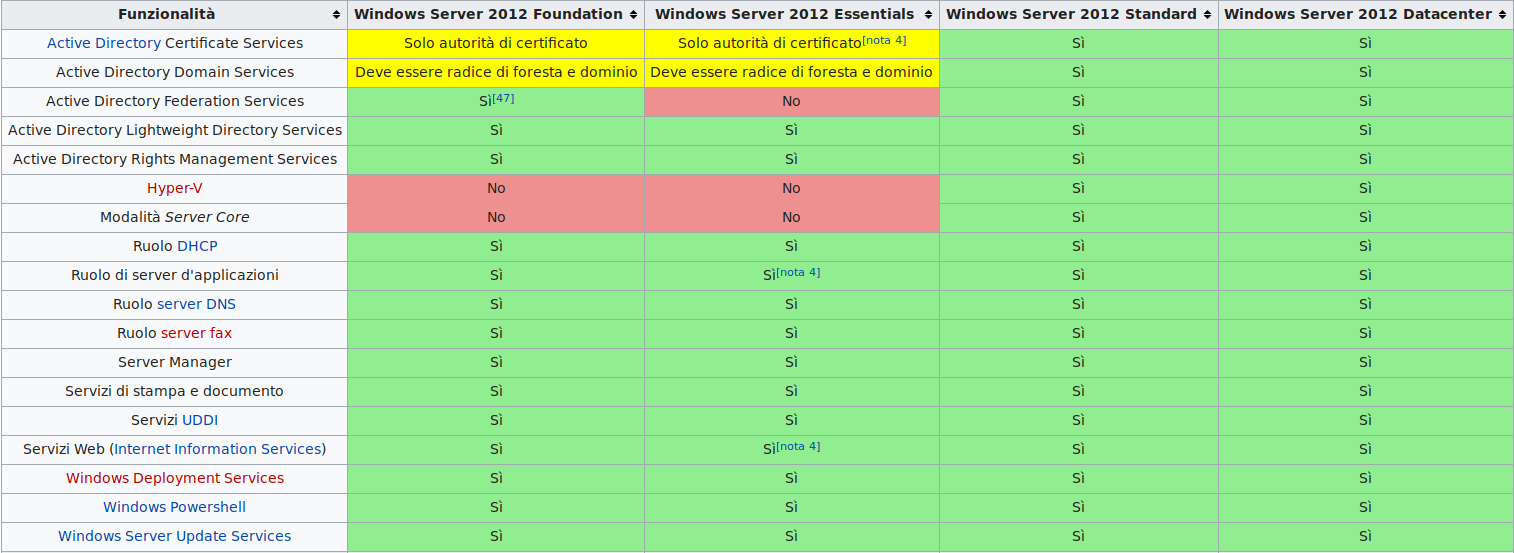
\includegraphics[scale=0.3]{images/tabecomp.png}
    \caption{Versioni Windows Server 2012}\label{fig:1}
\end{figure}

\subsection{Installazione di un sistema Windows 10}
\subsubsection{Versione utilizzata e requisiti minimi di sistema}
\textbf{Versione:} Windows 10 ???\\
\textbf{Memoria RAM:} 2 GB \\
\textbf{Hard Disk:} 60 GB

\subsection{Installazione di un sistema Linux}
\subsubsection{Versione utilizzata e requisiti minimi di sistema}
\textbf{Versione:} Kali Linux (con gnome) \\
\textbf{Memoria RAM:} 2048 MB \\
\textbf{Hard Disk:} 20 GB

\subsection{Impostazione avvio automatico}

\subsection{Configurazione disco di rete}

\textcolor{red}{NON ABBIAMO FINITO ANCORA, ALLO STATO ATTUALE ABBIAMO INSTALLATO LE MACCHINE VIRTUALI}

\end{document}
